\section{Einführung}
In diesem Versuch wird die optische Abbildung anhand einer digitalen Kamera untersucht.
Bei einer digitalen Kamera werden Gegenstände über Linsen auf einen Bildsensor (CMOS) abgebildet. Da die Abbildung am Rand der Linse deutlich schlechter wird, begrenzt man durch eine Blende mit Durchmesser $D$ den Lichtverlauf auf die Mitte.

\subsection{Auflösung}
Durch Beugungseffekte an der Blende werden auch Puntquellen nicht als Punkte, sondern als "Beugungsscheibchen" abebildet. Je größer der Durchmesser dieser Scheibchen, desto unschärfer wird das Bild. Das \emph{Rayleigh}-Kriterium besagt, dass zwei Punktquellen gerade noch unterscheidbar sind, wenn das Maximum der ersten mit dem 1. Minimum der zweiten Abbildung übereinanderliegt. Ein Beugungsscheibchen bei einer Wellenlänge $\lambda$ bei Linse mit Brennweite $f$ und Apertur $D$ hat den Durchmesser\footcite{anleitung-ss2015}
\begin{equation}
	d=2,4392...\cdot\lambda\cdot\frac{f}{D}
\label{eq:rayleigh}
\end{equation}
Der Wert 
\begin{equation}
	k=\frac{f}{D}
\label{eq:blendenzahl}
\end{equation}
heißt Blendenzahl.

\subsection{Schärfentiefe}
Da die digitale Kamera über eine oder mehrere Linsen im Objektiv abbildet, gibt es analog zur Brennweite einer Linse bei der Kamera eine Fokusentfernung $g$. Gegenstände, die den Abstand $g$ zur Kamera haben (sich in der Fokusebene befinden), werden mit maximaler Schärfe abgebildet. Ist ein Gegenstand näher oder weiter von der Kamera entfernt, verschlechtert sich die Schärfe. Der Nah- bzw. Fernpunkt ist der Punkt am nähesten bzw. am entferntesten zur Kamera, an dem ein Gegenstand noch ausreichend scharf abgebildet werden kann. Ausreichend scharf bedeutet, dass der Durchmesser der Zerstreuungskreise $Z$ einen bestimmten Wert nicht überschreitet (typischerweise $1/1500$ der Bilddiagonalen\footcite{anleitung-ss2015}). Ab einer bestimmten Fokusentfernung, der hyperfokalen Entfernung $d_h$, rückt der Fernpunkt ins Unendliche, d.h. scharfe Abbildung ist für beliebig weit hinter dem Nahpunkt liegende Gegenstände möglich.
\\
Die hyperfokale Entfernung beträgt

\begin{equation}
	d_h=\frac{f^2}{kZ}+f=f\cdot \left(\frac{D}{Z}+1\right)
\label{eq:hyperfok}
\end{equation}

Der Nahpunkt liegt bei 

\begin{equation}
	d_n=\frac{g(d_h-f)}{(d_h-f)+(g-f)}=\frac{g}{\frac{g-f}{d_h-f}+1}
\label{eq:nahpunkt}
\end{equation}

und der Fernpunkt bei

\begin{equation}
	d_f=\begin{cases}
		\frac{g(d_h-f)}{(d_h-f)+(f-g)}=\frac{g}{\frac{f-g}{d_h-f}} & g<d_h \\
		\infty & g \geq d_h
		\end{cases}
\label{eq:fernpunkt}
\end{equation}

\subsection{MTF}
Um die Auflösung quantitativ anzugeben, wird die Modulationsübertragunsfunktion MTF genutzt. Sei $\nu$ die Linienfrequenz eines Musters, d.h. die Dichte der Linien (Einheit z.B. Linienpaare pro Bildhöhe $lp/ph$). Ist $V_{\text{max}}$ der Grauwert des schwarzesten und $V_{\text{min}}$ der Grauwert des weißesten Pixels im Bild, so berechnet sich der Kontrast durch
\begin{equation}
	C(\nu)=\frac{V_{\text{max}}-V_{\text{min}}}{V_{\text{max}}+V_{\text{min}}}\qquad .
\label{eq:kontrast}
\end{equation}
Für $C(0)$ werden die Grauwerte bei einem vollständig schwarzen bzw. weißen Muster genommen. Dann ist die MTF das Kontrastverhältnis
\begin{equation}
	MTF(\nu)=C(\nu)/C(0)\qquad .
\label{eq:mtf}
\end{equation}
Eine Methode zur Messung der Linienpaaren ist der Siemensstern. In der Mitte des Sterns ist die Linienfrequenz so groß, dass nur noch eine graue Fläche abgebildet wird. Aus dem Durchmesser $d$ dieser Fläche und der Anzahl der Sektoren $n$ berechnet man die Auflösung in Linienpaaren
\begin{equation}
	l=\frac{n}{\pi d}\qquad .
\label{eq:siemens}
\end{equation}
\begin{figure}[h]
  \centering
  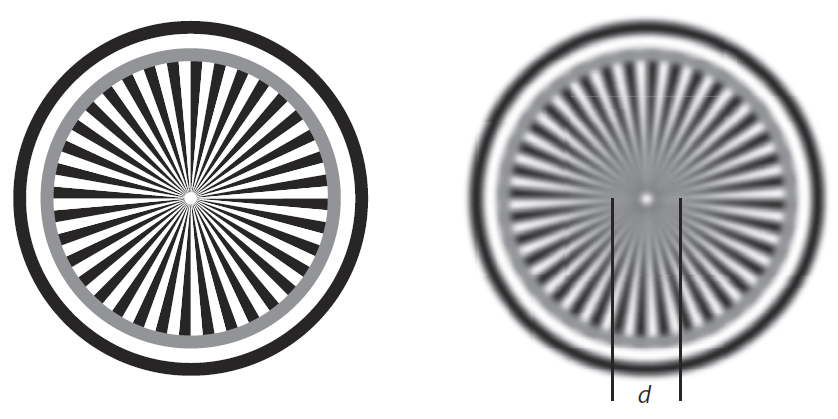
\includegraphics[width=.5\textwidth]{res/siemens}
  \caption{Siemensstern zur Bestimmung der Auflösung}
  \label{fig:siemens}
\end{figure}
Eine weitere Methode ist die der "schrägen Kante". Dabei wird ein Foto einer schrägen schwarzen Kante auf weißem Hintergrund aufgenommen. Aus dem Verlauf der Grauwerte an der Kante wird durch Differentiation und anschließende Fouriertransformation die MTF bestimmt.

\section{Versuche}
Die Kamera ist eine Nikon D3200 mit einem CMOS-Sensor der Größe $23.2 \times 15.4$ mm und einer Pixelzahl von $6016 \times 4000$ Pixel.
\subsection{Schärfentiefe}
Ein schräger Testchart mit aufgedrucktem Millimetermaß wird in $g=\SI{1.0(1)}{m}$ Entfernung bei verschiedenen Blendenzahen $k$ abfotografiert. Das Objektiv hat eine Brennweite von f=\SI{50}{mm}. Der Fokus wird am Anfang auf den Nullpunkt des Millimetermaßes eingestellt und dann nicht mehr geändert. Die Schärfentiefe wird am PC-Monitor subjektiv beurteilt und mit den theoretischen Werten aus \cref{eq:nahpunkt} bzw. \cref{eq:fernpunkt} gegenübergestellt. Dafür schätzen wir die Bildiagonale des Bildes auf dem Laptopbildschirm auf $d=\SI{36(3)}{cm}$, sodass sich für $Z$ der Wert $Z=d/1500=\SI{0.24(2)}{mm}$ ergibt.

\begin{table}[H]
  \centering
  \begin{tabular}{c | c |c c c} \toprule
		& subjektiv [\si{cm}]& \multicolumn{3}{c}{berechnet [\si{cm}]} \\ \midrule
    Blendenzahl $k$ & Schärfentiefe  & Nahpkt. $d_n$ & Fernpkt. $d_f$ & Schärfentiefe $\Delta d$\\ \midrule
    \num{1.8} & \num{4} & \num{84.89(730)} & \num{121.7(95)} & \num{36.81(1210)} \\
		\num{2.8} & \num{5.5} & \num{79.66(640)} & \num{134.3(88)} & \num{54.64(1091)} \\
		\num{4} & \num{6.5} & \num{73.24(550)} & \num{157.6(69)} & \num{84.36(885)} \\
		\num{5} & \num{8.5} & \num{68.65(490)} & \num{184.1(43)} & \num{115.5(65)} \\
		\num{8} & \num{15} & \num{57.78(380)} & \num{371.4(68)} & \num{313.6(684)} \\
		\num{9} & \num{15.5} & \num{54.98(350)} & \num{552.4(2133)} & \num{497.4(2133)} \\
		\num{10} & \num{19} & \num{52.26(330)} & \num{1156(1126)} & \num{1104(1126)} \\
		\num{11} & \num{20} & \num{49.92(310)} & $\infty$ & $\infty$ \\
		\num{13} & \num{22} & \num{45.75(280)} & $\infty$ & $\infty$ \\
		\num{14} & \num{25} & \num{43.92(270)} & $\infty$ & $\infty$ \\
		\num{16} & \num{26} & \num{40.66(250)} & $\infty$ & $\infty$ \\
		\num{18} & \num{28} & \num{37.87(230)} & $\infty$ & $\infty$ \\
		\num{20} & \num{28} & \num{35.42(220)} & $\infty$ & $\infty$ \\
		\num{22} & \num{28} & \num{33.24(200)} & $\infty$ & $\infty$ \\ \bottomrule 
  \end{tabular}
  \caption{Schärfentiefe $\Delta d$: subjektive und berechnete Werte}
  \label{tab:schaerfentiefe}
\end{table}

Zu sehen ist, dass qualitativ die Schärfentiefe mit der Blendenzahl steigt, was sich sowohl in den subjektiven als auch den berechneten Werten niederschlägt. Allerdings ist die berechnete Schärfentiefe deutlich größer als die subjektive. Außerdem steigen die berechneten Werte schneller mit der Blendenzahl: Während der erste Wert ca. viermal so groß ist wie der subjektive, ist die berechnete Schärfentiefe zur Blendenzahl \num{10} schon ca. 50 mal größer.

Es fällt der große Fehler bei den Blendenzahlen 9 bzw. 10 auf. Der Grund ist, dass hier die Gegenstandsweite nahe an der hyperfokalen Entfernung liegt, diese aber noch nicht überschritten hat. Für diese Werte ist \cref{eq:fernpunkt} sehr empfindlich gegenüber Unsicherheiten in der Gegenstandsweite.

Ab Blendenzahl \num{11} ist die hyperfokale Entfernung größer als die Fokusentfernung, sodass der Fernpunkt ins Unendliche rückt und die theoretische Schärfentiefe unendlich groß ist. Die subjektive Schärfentiefe nahm jedoch noch weiter zu, erreichte aber ab Blendenzahl \num{18} das Ende der aufgedruckten Skala.

\subsection{MTF}
Nun wurde mittels eines ImageJ-Plugins, welches das "schräge Kante"-Verfahren nutzt, die Linienfrequenz (lp/mm) ermittelt, bei der die MTF auf 0.5 abfällt. Dies wurde für jede Blendenzahl wiederholt.
\iffalse
\begin{table}[H]
  \centering
  \begin{tabular}{c c c c c} \toprule
    Blendenzahl $k$ & Linienfrequenz bei MTF=0.5 \si{lp/mm} \\ \midrule
    \num{1.8} & \num{4} \\
		\num{2.8} & \num{5.5} \\
		\num{4} & \num{6.5} \\
		\num{5} & \num{8.5} \\
		\num{8} & \num{15} \\
		\num{9} & \num{15.5} \\
		\num{10} & \num{19} \\
		\num{11} & \num{20} \\
		\num{13} & \num{22} \\
		\num{14} & \num{25} \\
		\num{16} & \num{26} \\
		\num{18} & \num{28} \\
		\num{20} & \num{28} \\
		\num{22} & \num{28} \\ \bottomrule 
  \end{tabular}
  \caption{MTF-Abfall auf 0.5 für verschiedene Blendenzahlen}
  \label{tab:mtf}
\end{table}
\fi

\begin{figure}[H]
\centering
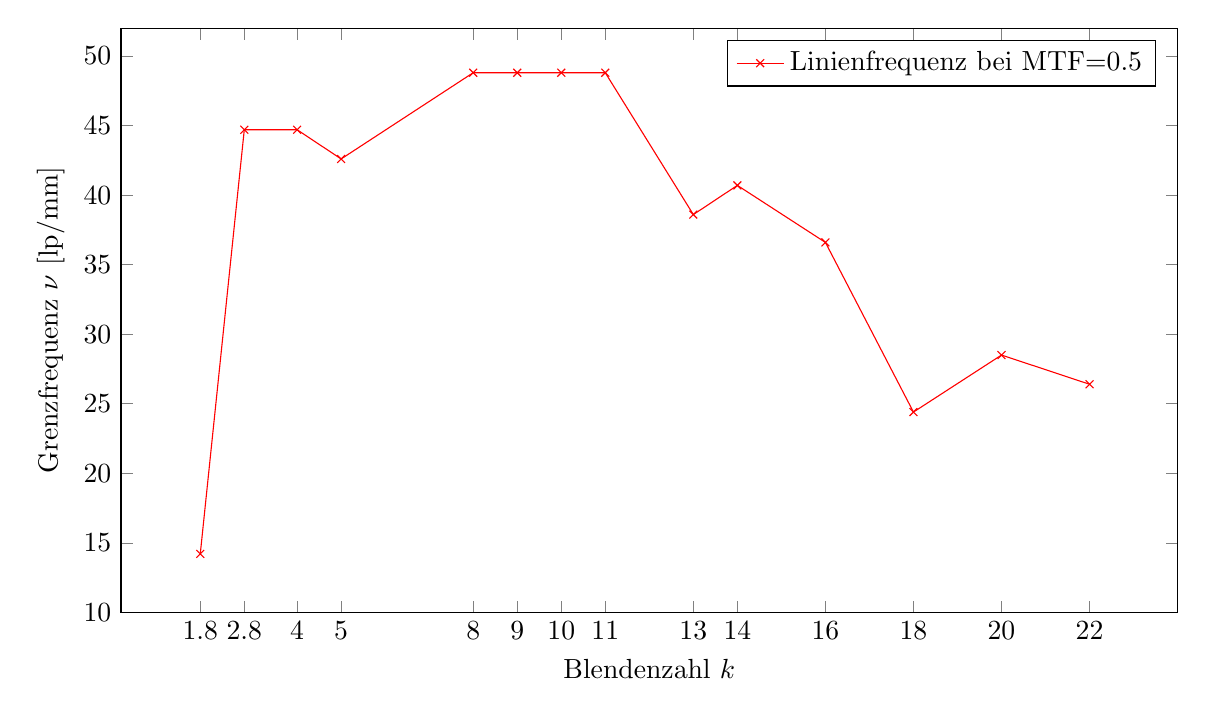
\begin{tikzpicture}
  \begin{axis}[
    width=15 cm,
    height=9 cm,
    xmin=0, xmax=24,
    ymin=10, ymax=52,
    xlabel={Blendenzahl $k$},
    ylabel={Grenzfrequenz $\nu$ [\si{lp/mm}]},
    domain=0:24,
    cycle list name=color list,
    legend entries={Linienfrequenz bei MTF=\num{0.5}},
		xtick=data
  ]
  \addplot+ plot [mark=x]  table{
		1.8	14.2
		2.8	44.7
		4		44.7
		5		42.6
		8		48.8
		9		48.8
		10	48.8
		11	48.8
		13	38.6
		14	40.7
		16	36.6
		18	24.4
		20	28.5
		22	26.4
	};
  \end{axis}
\end{tikzpicture}
\caption{Linienfrequenz $\nu$, bei der die MTF auf \num{0.5} abgefallen ist, in Abhängigkeit der Blendenzahl $k$}
\label{fig:mtf}
\end{figure}

Es sind keine Fehlerbalken eingetragen, weil nicht genügend Informationen zum Plugin bekannt sind. Qualitativ ist zu sehen, dass die Grenzfrequenz bei der kleinsten Blendenzahl $k=\num{1.8}$ im Vergleich sehr niedrig liegt (\SI{14.2}{lp/mm}). Der zweite Wert liegt deutlich höher bei $\nu=\SI{44.7}{lp/mm}$. Ab hier ist ein leichter Anstieg auf $\nu=\SI{48.8}{lp/mm}$ erkennbar, der aber im Bereich des Fehlers liegen könnte. Anschließend verzeichnet sich grob gesehen mit zunehmender Blendenzahl ein Abfall in der Grenzfrequenz, wobei die Ausreißer bei $k=13$ bzw. $k=18$ auf Messunsicherheiten zurückzuführen sein könnten. Die Grenzfrequenz der größten Brennzahl liegt ungefähr auf der Hälfte des Maximalwertes, ist aber immer noch knapp doppelt so hoch wie der kleinste Wert.

\section{Diskussion}

\subsection{Schärfentiefe}

Bei der Schärfentiefe ist ein großer quantitativer Unterschied zwischen subjektiven und berechneten Werten aufgetreten (z.B. $k=\num{1.8}$, subjektiv: \SI{4}{cm}, berechnet: \SI{37}{cm}). Grund dafür ist, dass bei der subjektiven Beobachtung nicht bekannt war, wie ein Übergang von scharf zu unscharf bei $Z=\text{Bilddiagonale}/1500$ aussieht. Außerdem war bei größeren Blendenzahlen der subjektive Fernpunkt schon über die Skala hinausgelaufen, während der (subjektive) Nahpunkt noch auf der Skala lag. Für diese Werte haben wir den Maximalwert der Skala als Fernpunkt angenommen, was natürlich zu klein ist.

Außerdem sind die Fehler der berechneten Werte (außgenommen $k=9, k=10$) zwar noch akzeptabel, aber größer als gewünscht. Man hätte den Fokusabstand $g$ und die Bilddiagonale $g$ am Laptopbildschirm genauer messen müssen, um hier auf exaktere Werte zu kommen. Der explodierende Fehler der letzten beiden Blendenzahlen vor der hyperfokalen Entfernung ist auf die schlechte Konditionierung der Fernpunktsgleichung~\cref{eq:fernpunkt} in der Nähe von $d_h$ zurückzuführen.\\

Qualitativ bestätigt jedoch die subjektive Beobachtung die Theorie insofern, als dass eine höhere Blendenzahl zu einer höheren Schärfentiefe führt.

\subsection{MTF}
Die Grenzfrequenz gibt an, wie dicht Linienpaare in einem Muster aneinander liegen können bevor der Kontrast $\SI{50}{\percent}$ des Maximalkontrastes unterschreitet. Also entspricht eine höhere Grenzfrequenz einer genaueren Auflösung. Aus dem Rayleigh-Kriterium (vgl. \cref{eq:rayleigh}) wird erwartet, dass die Auflösung umso genauer ist, desto kleiner die Blendenzahl ist. Deshalb erwarten einer Abnahme der Grenzfrequenz mit zunehmender Blendenzahl.\\

Diese Erwartung ist innerhalb von Messfehlern mit den Ergebnissen vereinbar, wenn man den Wert für $k=1.8$ herausnimmt. Ein möglicher Grund für die schlechte Auflösung bei dieser Blendenzahl könnten Linsenfehler sein: Die kleinste Blendenzahl entspricht der größtmöglichen Blendenöffnung, d.h. das einfallende Licht passiert möglicherweise den Rand der Linsen im Objektiv, der anfälliger für Linsenfehler ist. Dadurch könnte sich die Auflösung verschlechtert haben.
